% placeholder-figure.tex — a neutral stand-in figure shipped with the template.
%
% Purpose: the demo \housefigure/\includegraphics calls in writing/ point here on a
% freshly scrubbed project, so `make paper`/`make slides` compile green before any real
% analysis output exists. Replace with your own output/figures/... and repoint the doc.
%
% Standalone; compile with lualatex to regenerate placeholder-figure.pdf:
%     lualatex placeholder-figure.tex
\documentclass[border=2pt]{standalone}
\usepackage{tikz}
\begin{document}
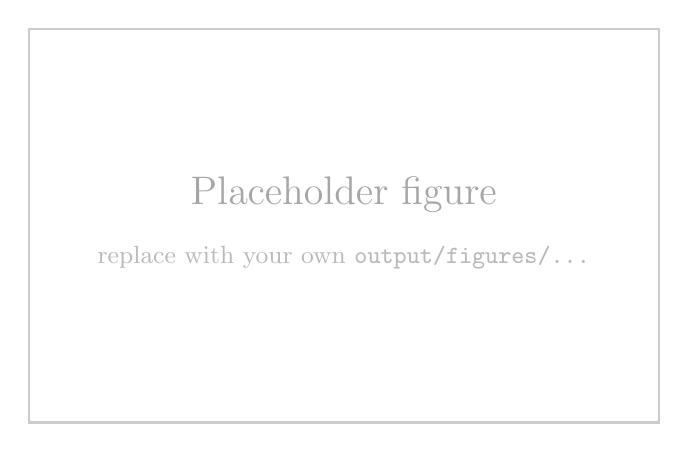
\begin{tikzpicture}
  \draw[gray!40, line width=0.8pt] (0,0) rectangle (8,5);
  \node[gray!70] at (4,2.9) {\Large Placeholder figure};
  \node[gray!55] at (4,2.1) {\small replace with your own \texttt{output/figures/\ldots}};
\end{tikzpicture}
\end{document}
